\documentclass[final]{fhnwreport}       %[mode] = draft or final
                                        %{class} = fhnwreport, article, 
                                        %          report, book, beamer, standalone
\usepackage{hyperref}
\usepackage{longtable} % To display tables on several pages
\usepackage{lipsum}
\usepackage{silence}
\WarningFilter{hyperref}{Draft mode on}
\WarningFilter{latex}{Marginpar}
\usepackage{graphicx}

% Load the package
\usepackage[toc]{glossaries}
% Generate the glossary
\makeglossaries

%%---Main Packages-----------------------------------------------------------------------
\usepackage[english, ngerman]{babel}	%Mul­tilin­gual sup­port for LaTeX
\usepackage[T1]{fontenc}				%Stan­dard pack­age for se­lect­ing font en­cod­ings
\usepackage[utf8]{inputenc}				%Ac­cept dif­fer­ent in­put en­cod­ings
\usepackage{lmodern}                    %The newer Font-Set
\usepackage{textcomp}					%LaTeX sup­port for the Text Com­pan­ion fonts
\usepackage{graphicx} 					%En­hanced sup­port for graph­ics
\usepackage{float}						%Im­proved in­ter­face for float­ing ob­jects
\usepackage{ifdraft}                    %Let you check if the doc is in draft mode

%%---Useful Packages---------------------------------------------------------------------
\usepackage[pdftex,dvipsnames]{xcolor}  %Driver-in­de­pen­dent color ex­ten­sions for LaTeX
\usepackage{csquotes}                   %Simpler quoting with \enquote{}
\usepackage{siunitx} 					%A com­pre­hen­sive (SI) units pack­age
\usepackage{listings}					%Type­set source code list­ings us­ing LaTeX
\usepackage[bottom]{footmisc}			%A range of foot­note op­tions
\usepackage{footnote}					%Im­prove on LaTeX's foot­note han­dling
\usepackage{verbatim}					%Reim­ple­men­ta­tion of and ex­ten­sions to LaTeX ver­ba­tim
\usepackage[textsize=footnotesize]{todonotes} %Mark­ing things to do in a LaTeX doc­u­ment

%%---Tikz Packages-----------------------------------------------------------------------
\usepackage{standalone}
\usepackage{tikz}
\usepackage{circuitikz}
\usetikzlibrary{arrows}
\usetikzlibrary{calc}
\usetikzlibrary{intersections}

%%---Math Packages-----------------------------------------------------------------------
\usepackage{amsmath}					%AMS math­e­mat­i­cal fa­cil­i­ties for LaTeX
%\usepackage{amssymb}					%Type­set­ting symbols (AMS style)
%\usepackage{array}						%Ex­tend­ing the ar­ray and tab­u­lar en­vi­ron­ments
%\usepackage{amsthm}					%Type­set­ting the­o­rems (AMS style)

%%---Table Packages----------------------------------------------------------------------
\usepackage{tabularx}					%Tab­u­lars with ad­justable-width columns
%\usepackage{longtable}
\usepackage{multirow}					%Create tab­u­lar cells span­ning mul­ti­ple rows
\usepackage{multicol}					%In­ter­mix sin­gle and mul­ti­ple columns

%%---PDF / Figure Packages---------------------------------------------------------------
\usepackage{pdfpages}					%In­clude PDF doc­u­ments in LaTeX
\usepackage{pdflscape}					%Make land­scape pages dis­play as land­scape
\usepackage{subfig}					    %Fig­ures di­vided into sub­fig­ures

%%---Other Packages----------------------------------------------------------------------
%\usepackage{xargs}                     %De­fine com­mands with many op­tional ar­gu­ments

%%---Bibliography------------------------------------------------------------------------
\usepackage[style=ieee,urldate=comp,backend=biber]{biblatex}
\addbibresource{literature/bibliography.bib}

%%---Main Settings-----------------------------------------------------------------------
\graphicspath{{./graphics/}}			%Defines the graphicspath
\geometry{twoside=false}				    %twoside=false disables the "bookstyle"
\setlength{\marginparwidth}{2cm}
\overfullrule=5em						%Creates a black rule if text goes over the margins => debugging




%%---User Definitions--------------------------------------------------------------------
%%Tabel-Definitions: (requires \usepackage{tabularx})
\newcolumntype{L}[1]{>{\raggedright\arraybackslash}p{#1}}    %column-width and alignment
\newcolumntype{C}[1]{>{\centering\arraybackslash}p{#1}}
\newcolumntype{R}[1]{>{\raggedleft\arraybackslash}p{#1}}

%%---Optional Package Settings-----------------------------------------------------------
%Listings-Settings: (requires \usepackage{listings}) => Example with Matlab Code
\lstset{language=Matlab,%
    basicstyle=\footnotesize\ttfamily,
    breaklines=false,%
    morekeywords={switch, case, otherwise},
    keywordstyle=\color{Blue},%
    tabsize=2,
    %morekeywords=[2]{1}, keywordstyle=[2]{\color{black}},
    identifierstyle=\color{Black},%
    stringstyle=\color{Purple},
    commentstyle=\color{Green},%
    showstringspaces=false,%without this there will be a symbol in the places where there is a space
    numbers=left,%
    numberstyle={\tiny \color{black}},% size of the numbers
    numbersep=9pt, % this defines how far the numbers are from the text
    %emph=[1]{word1, word2,...},emphstyle=[1]\color{red}
}							                            %loads all packages, definitions and settings, except bibliography (otherwise vim-latex doesn't recognise for completion)

%%---Bibliography------------------------------------------------------------------------
%% \usepackage[style=ieee,urldate=comp,backend=biber]{biblatex}
%% \addbibresource{literature/bibliography.bib}

\usepackage[natbib=true, citestyle=apa, bibstyle=apa]{biblatex}
\bibliography{literature/bibliography.bib}


\title{Effectivenes simulation of a rebalancing algorithm for the Lightning Network under partial participation}                          %Project Title
\author{Bachelor Thesis}                %Document Type => Technical Report, ...
\date{August 1, 2020}                   %Place and Date

\begin{document}
%%---TITLEPAGE---------------------------------------------------------------------------
\selectlanguage{english}                %ngerman or english
\maketitle

\vspace*{-1cm}                            %compensates the space after the date line.
\vfill
{
\renewcommand\arraystretch{2}
\begin{center}
\begin{tabular}{>{\bf}p{4cm} l}
Organization                  &    FHNW, School of Business, Basel\\
Study program                 &    Business Information Technology\\
Author                        &    Tobias Koller\\
Supervisor                    &    Prof. Dr. Kaspar Riesen\\
Project sponsor               &    Prof. Dr. Thomas Hanne\\
Expert                        &    René Pickhardt
\end{tabular}
\end{center}
}
\clearpage

%% -- ABSTRACT
\thispagestyle{empty}
\begin{abstract}
  Here follows my abstract
  \lipsum{1-2}

  \vspace{2ex}
  \textbf{Keywords: Lightning, Bitcoin, path finding}
\end{abstract}
\vfill

%%---TABLE OF CONTENTS-------------------------------------------------------------------
\pagenumbering{Roman}		
\tableofcontents
\clearpage

%%---DECLARATION OF HONOR
\addcontentsline{toc}{section}{Declaration of honor}
\vfill\noindent
\begin{center}
 \section*{DECLARATION OF HONOR}
\end{center}

I the undersigned declare that all material presented in this paper is my own work or fully and specifically acknowledged wherever adapted from other sources. I understand that if at any time it is shown that I have significantly misrepresented material presented here, any degree or credits awarded to me on the basis of that material may be revoked. I declare that all statements and information contained herein are true, correct and accurate to the best of my knowledge and belief. This  paper or part of it have not been published to date. It has thus not been made available to other interested parties or examination boards.  

\vspace*{4em}\noindent
\hfill%
\begin{tabular}[t]{c}
  \rule{10em}{0.4pt}\\Tobias Koller 
\end{tabular}%
\hfill%
\begin{tabular}[t]{c}
  \rule{10em}{0.4pt}\\ Place / Date
\end{tabular}%
\hfill\strut
\clearpage

%%---FOREWORD
\section*{Foreword}
\addcontentsline{toc}{section}{Foreword}
\todo[inline]{Some background}
\clearpage

%%---GLOSSARY
\clearpage


\pagenumbering{arabic}
\section{Introduction} 
This section gives a brief introduction and overview of the Bitcoin and Lightning technology. It covers the history of digital cash, the advent of Bitcoin and explains the need for an off-chain scaling solution. 

\subsection{Bitcoin: Peer to Peer Electronic Cash}\label{subsec:peertopeer}
Bitcoin is a peer-to-peer electronic cash system first introduced in a white paper by the individual or group behind the pseudonym Satoshi Nakamoto \citep{nakamoto_bitcoin_2008}. This paper lines out the fundamental principles of the Bitcoin block chain \todo{glossary block chain} that achieves digital transfer of value without a central third party. The next paragraph expands on the pre-bitcoin developments on electronic cash that eventually lead to the rise of Bitcoin. Additionally, we explain why there is a need for additional layer protocols.

\subsubsection{History of digital cash}
Before the digital age cash was the dominant form of payment. A bank note or a coin embodies the respective face value to the bearer of it. Economical transactions can be made by simply exchanging this physical token by which the transaction was immediately settled. However, with the advent of e-commerce this simple and transparent mechanism was no longer possible. New institutions formed to fulfill the need of online transactions. Credit card companies and payment processors filled the gap of trust needed between the sender and the receiver of a transaction over the internet. This architecture came with significant drawbacks. Suddenly, the interacting parties are dependent on third parties which are collecting additional fees. Use of such systems require identification and since the intermediary can track all transactions, this reduces the user's privacy \citep{narayanan_bitcoin_2016}.

Bitcoin is by no means the first system introduced to allow for a digital cash system. Already in in 1983 \citeauthor{chaum_blind_1983} worked on new cryptographic primitives that should make electronic banking services more private and offer improved auditability \citep{chaum_blind_1983}. Although his technology still relied on a central ``bank'' server which issues electronic bills, blinded signatures allowed to anonymously transfer them. In 1989 the company \textbf{DigiCash} was found by Chaum to commercialise the idea and a few banks did later implement it. Technological complexity, patents on the invention and the incapability of handling  user-to-user transactions prevented it from becoming a success \cite{narayanan_bitcoin_2016}. 

An important problem in the evolution of digital cash has been the so called \textbf{\gls{doublespend}}. Digital information has the property of being easily duplicated. This poses a problem to digital cash as this behaviour is generally unwanted. How can a receiver of digital cash be certain that the cash has not been spent to someone else before, thus eliminating its value? Satoshi Nakamoto introduced the concept of a global distributed ledger, a data structure that is append only and where any change must be disseminated to all participants. In order to keep the history of the ledger immutable Satoshi utilizes the idea of a time stamping server first proposed by \textcite{haber_how_1991} in 1991. It works by calculating the hash of a piece of data and publishing it to all the participants. This serves as a proof that the data existed at this given time since otherwise the hash could not have been calculated. The next piece of data to be published also contains the previous hash, effectively linking them and forming a chain. If someone would now want to change the underlying data this would change its hash and since it is included in the next element in the chain also this hash would need to be changed up until the most recent element. 
\todo[inline]{explain hash and add to glossary}

Maintaining a global state of transactions in a constantly changing network of participants which can not be trusted is challenging. A single user could spin up hundreds of nodes to overcome the conses of the network. How can a consensus be formed without a central authority? A solution to a similar problem was proposed by \textcite{back_hashcash_2002} in 2002. To prevent e-mail spamming he introduced a mechanism that requires the sender to solve a puzzle that is computational heavy. This so called ``proof of work'' is requested by the receiver of the e-mail to trust that it is no spam. Since this computation can easily be done for one e-mail it becomes a big burden to do for thousand of e-mails therefore avoiding spammers. The puzzle simply involves finding a value whose hash starts with a certain amount of zero bits. Since the result of a hash function can not be predicted only brute force can be applied to find such a value. By selecting the number of leading zero bits one can change the difficulty of the puzzle. Each additional zero leads to the difficulty to be doubled. In order to add transactions to the Bitcoin ledger a participant constructs a block consisting of transactions, computes the proof of work and publishes it to the network. Only if all transactions are valid and the work done has been verified network participants append the transactions to their local copy of the ledger and further broadcast the block.  
\todo[inline]{add pow to glossary}

Combining proof of work with the chaining of hashes introduced in the last paragraph results in a strong security model. An attacker who wants to change the history of the ledger would need to recompute the proof of work of the changed and all subsequent blocks as they are linked by their hashes. Therefore, every new block makes it increasingly more difficult to change a transaction in the ledger. Number of blocks on top of a transaction in question is hence be referred to as \textbf{confirmations}.  

\subsubsection{Scaling solutions}
One of Bitcoin's value propositions is being decentralised. At the same time every transaction ever made must be distributed and stored among all network peers. It becomes obvious that some trade-off has to be made to maintain those two properties: scalability. This is often referred to as the scalability trilemma \todo{trillema in glossary} which states that in distributed systems the three objectives \textbf{security}, \textbf{decentralisation} and \textbf{scalability} can not be achieved in full extent at the same time. While two can often be achieved, there are certain trade-offs to be made in the third domain. This section is explaining why this is true for Bitcoin and what main categories of solution exist.

While decentralisation can be described on many levels we focus here on the decentralisation of validating nodes. Those are network participants that verify the blocks published by miners. Decentralisation would be best achieved if  every user of Bitcoin would run its own fully validating node \todo{add full node to glossary}to receive information about the ledger independently. On the other hand the network would be centralised when only few nodes would validate and users would need to trust those to tell the truth about the ledger state. To keep decentralisation high it is crucial to keep the hardware and network requirements as low as possible. The Bitcoin protocol restricts the amount of data to be processed to one block of 1 megabyte per 10 minutes. A full node in the network must be able to download at least 1 MB / 10 minutes in order to keep up with the tip of the chain. Lower bandwidth would cause it to get left behind without every being able to catch up. Additionally, the full node must keep the full ledger on storage. This yields to approximately 286 GB \cite{noauthor_blocks-size_nodate} at time of writing, increasing linearly in the future. This upper limit block size results in a throughput of approximately 7 transactions per second (tps) \cite{poon_bitcoin_2016}. Clearly by several orders of magnitude smaller than what it would require to become a world wide payments network. 

Bitcoin, by design, promotes security and decentralisation while sacrificing scalability. However, to be usable by everyone the scalability issue needs to be addressed. As Bitcoin is not owned by anyone there is no one party to decide on the future design decisions. This lead to a scaling debate with two ideological camps on how to progress. Scaling on-chain or scaling off-chain.

Scaling on-chain means lifting the 1 megabyte block limit, allowing for a higher transaction throughput. While this seems the most straight forward solution it can not be achieved without trade-off. As previously discussed decentralisation can only be maintained by keeping the hardware and network requirements low. Removing this restriction to allow worldwide usage would mean that nodes soon need to process hundreds of megabytes or even gigabytes per second, effectively reducing the number of nodes that can still keep up, leading to a more centralised network. 

An off-chain scaling solution describes any system that acts outside of the Bitcoin protocol but is linked to it, in a way that leverages the number of economical transactions that can be performed per single on-chain transaction. These solutions build a second layer \todo{glossary second layer} of abstraction. While still using functionality of the base layer \todo{glossary base layer} they can reduce their dependency and make their own design decisions and trade-offs based on the scalability trilemma. The Lightning Network is only one possible off-chain solution and is described in the next section in more depth. 

\subsection{Lightning technology}
The Lightning Network is a network protocol that utilizes Bitcoin as its underlying trust system. It can, therefore, be described as a ``second layer'' protocol building upon the Bitcoin ``base layer''. Bitcoin does not scale on the base layer since it was designed with security and decentralisation in mind. Off-chain solutions like Lightning are developed to facilitate more transactions on a different layer without compromising the properties of the base layer \citep{poon_bitcoin_2016}.

% The Bitcoin system consists of nodes each maintaining a ledger of historic transactions. All new transactions must be distributed to all nodes and validated by them. Transactions are therefore public information and must be stored by all nodes. To allow many people to run a node, therefore promoting a decentralized network, the hardware requirements must be as low as possible. This is why there is a limitation of new transactions that can be recorded in the network causing this low transaction throughput.
\subsubsection{Payment channels}
The transaction bottleneck in Bitcoin is imposed since every network participant needs to be updated about every transaction. This is required to ensure the integrity of the system and not because the transactions are of interest to the nodes. In fact they can learn very little about the parties involved in a transaction as pseudonymous public keys are used as identifiers. \citeauthor{poon_bitcoin_2016} mention in the Lightning Network Paper that as long as only two participants care about a recurring transaction there is no need to inform the entire network about it \citep{poon_bitcoin_2016}. They therefore propose that those two participants do not sent the transaction to the network but instead hold on to it and agree on their balances bilaterally. \textquote[{\cite{poon_bitcoin_2016}}, p. 4]{Micropayment channels create a relationship between two parties to perpetually update balances, deferring what is broadcast to the block chain in a single transaction netting out the total balance between those two parties.}

Opening such a payment channel requires the two parties to create an on-chain Bitcoin transaction which spends an amount of bitcoin to a 2-of-2 multisignature contract. Only both parties collaboratively can spend it from there. At the same time they create a refund transaction that spends from the multisignature contract and distributes the current balance state. However, they could broadcast this transaction instead they can also decide to hold on to it and update it at a later stage. Holding the signed Bitcoin transaction ensures that they could at any time get their balance back on-chain. Every time they wish to transact with each other they just sign a new refund transaction which distributes the updated channel balance.

\textit{Example:} Assume Alice and Bob open a payment channel and both send 0.5 BTC to a 2-of-2 multisignature contract. This channel has a total capacity of $0.5 + 0.5 = 1$ BTC. At the same time they also create a transaction that pays them back their initial balance of 0.5 BTC each. This transaction is not sent to the block chain but kept private by the two parties. If Alice wants to send Bob 0.2 BTC they update this transaction spending the initial 1 BTC to be distributed as follows: 0.3 BTC to Alice; 0.7 BTC to Bob. This payment was only agreed upon Alice and Bob, no one else needed to be notified. Unlimited future transactions like this can take place as long as the sender still has some balance. At any point in time Alice or Bob can decide to broadcast the latest transaction, distributing the agreed balance and effectively closing the payment channel. As depicted in figure~\ref{fig:ChannelCycle} there can be many modifications to that balance.

\begin{figure}[H]
\centering
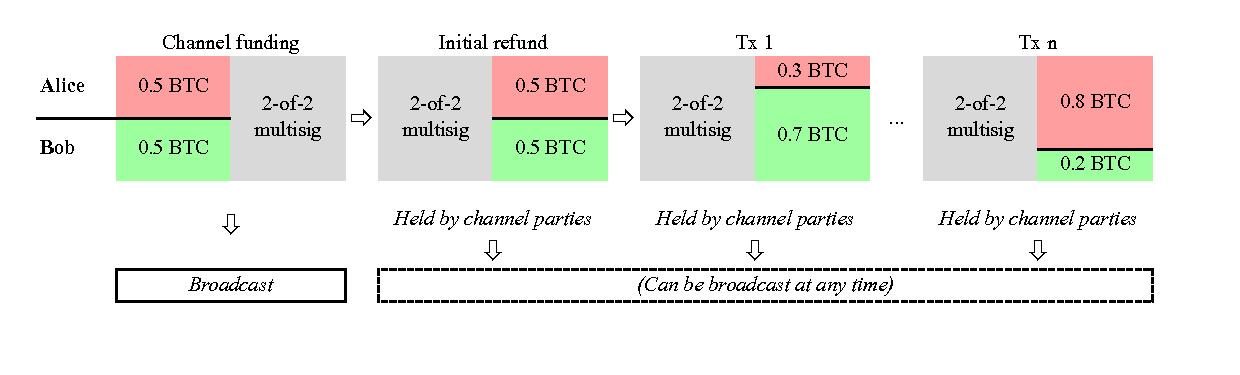
\includegraphics[width=0.9\linewidth]{channel_lifecycle.pdf}
\caption{Life cycle of payment channel.}
\label{fig:ChannelCycle}
\end{figure}

Transactions within these channels are only visible to the two partners but stay invisible to the rest of the network. While opening and closing a channel each requires one transaction in the base layer (Bitcoin) unlimited transactions with almost no throughput restriction can be facilitated within a channel during its lifetime. 

It is important to note the difference between a Lightning node and a Bitcoin node. While they can run on the same system, they operate in two different networks. A Bitcoin node works well individually but a Lightning node needs to have access to a Bitcoin node.

For a node to pay another node that it has no direct channel open with, he can simply route the transaction via other nodes and their channels. Since the network graph is public, the path can be chosen by the initiator of a transaction. This is called source routing. 

A payment channel is always opened between two nodes. One of the participants acts as the initiator and provides funds for the channel in the form of bitcoin. This leads to the total capacity being allocated to his or her balance within the channel. As soon as he starts to make payments towards the other node, his or her balance decreases, and the partner's balance increases (total capacity remains constant). Transactions can only be executed if the amount is smaller or equal than the channel's capacity and if the sending node has enough local balance. Channels and their capacities are announced to the network but the distribution of balances remains private to the channel partners.

\subsubsection{Source Routing}
explain source routing

\newpage
\section{Problems in graph theory}
\todo[inline]{Go from general graph theory problems into more specific areas, 1 paragraph per topic}
\todo[inline]{Explain why finding a path in the lightning network can be so difficult}
\subsection{Overview of broad problems}
one paragraph per
\begin{itemize}
  \item coloring
  \item enumeration
  \item subgraphs
  \item route problems (explained more depth)
  \item network flow (explained more depth)
\end{itemize}

\subsection{Route problems}
kd
\subsection{Network flow}
kdf

\subsection{Application in the Lightning Network}
\todo[inline]{problem to be solved in ln is network flow: find route that accommodates enough liquidity without knowing the balances. In experiment algorithm does rebalancing by trying to reallocate funds differently (greedy)}

Nodes trying to find a path in the Lightning Network work with limited information. While they know what channels are available and what their capacities are, they do not know about the balances and therefore whether the nodes can forward their payment or not. Hence, it is likely that a payment attempt fails because a node had insufficient balance. The paying node needs to find another route and retry the payment until it succeeds. If the payment fails repeatedly it can cause delays that are bad for the user experience. 

\subsection{Problem statement}
\todo[inline]{Only give a brief informal overview of the problem but forward reference to the next chapter}

These payment channel networks are decentralized by nature and no protocol change can be forced upon the node operators. Therefore, the question arises on how effective this protocol change will be assuming only partial participation of nodes. What are the effects of different levels of participation on the imbalance measure \footnote{Defined as the inequality of the distribution of a nodes channel balance coefficients} of the network during repeated rebalancing cycles? What is the effect of different levels of participation on the network's ability to route payments between random nodes? 

\subsection{Previous work}
René Pickhardt's and Mariusz Nowostawski's publication ``Imbalance measure and proactive channel rebalancing algorithm for the Lightning Network'' \cite{pickhardt_imbalance_2019} serves as a base to formulate the question for this thesis. In their work, they present a solution for the pathfinding problem in a privacy-aware payment channel network. The proposed solution includes a rebalancing protocol which the nodes of the network should follow to achieve a higher balancedness (for itself but also the entire network). It consists of instructions to proactively rebalance their channels within their friend of a friend's network, redistributing the relative funds owned in a channel but leaving total funds owned unchanged.

Rebalancing is an activity where one node engages in a circular payment that pays itself. This is only possible when the node has at least two channels with different peers. The payment gets routed \textbf{out} through one channel and is \textbf{received back} over another. On the way, it can use one or more hops to find back to the sender node. This procedure enables a node to change the balances of the individual channels while the total node balance stays the same. In practice, there would be a fee collected by the intermediate nodes whose channels are used. In the proposed rebalancing protocol nodes would forego the fee and only participate in the rebalancing attempt if their balancedness improves as well.

\section{Experiment} \label{sec:method}
\todo[inline]{explain all the performance measures}
\todo[inline]{explain methodology}
\todo[inline]{explain the experimental setup}
\subsection{Preprocessing}
\todo[inline]{explain which nodes and channels where selected}

\subsection{Lightning properties}
%% Dummy text

\subsection{Implementing routing protocol}
\todo[inline]{Describe how the proposed protocol change is impolemented in the \textbf{Network} class. }
\todo[inline]{show illustrations with a dummy network}
\todo[inline]{ask Rene to his dummy network}

\subsection{Methodology}
\todo[inline]{explain how to get the network information for a running node. quickly show how I extracted the data from the full node. Explain the structure of the python class \textbf{Network}}. And some more \textbf{bold text}.

To model the network, public information from the Lightning Network is used. From a Lightning node, all the channel and node information can be extracted.

For all further manipulations and calculations, the programming language Python will be used. This includes writing code that facilitates: 
\begin{itemize}
  \item The selection of nodes, participating in the protocol change.
  \item Implement the proposed algorithm \cite[p.~3]{pickhardt_imbalance_2019}.
  \item Performing rebalancing in the network.
  \item Storing different network states for different scenarios.
  \item Calculate different performance measures.
  \item Aggregate data.
  \item Plot graphs to visualize the results.
\end{itemize}


\section{Results}
%% Dummy text
\section{Conclusion \& Outlook}
%% Dummy text

%%---BIBLIOGRAPHY------------------------------------------------------------------------
\newpage
{\sloppypar
\addcontentsline{toc}{section}{Bibliography}
\printbibliography
\label{sec:lit}
}


%Print the glossary
\newpage
\newglossaryentry{doublespend}{name={double spend problem}, description={Problem in digital cash systems that a digital token can be duplicated at will and used as payment to multiple receivers at the same time making it difficult to detect the fraud.}}
\section*{Glossary}
\printglossaries

\appendix
\section{Some appendix}
maybe\ldots

%%---TODO-OVERVIEW-------------------
\ifdraft{%Do this only if mode=draft
\newpage
\listoftodos[\section{Todo-Notes}]
\clearpage
}
{%Do this only if mode=final
}

\end{document}

